\chapter{評価}
\label{chap:kekkahyouka}

\section{RQ1:レビューの抽出性能はどの程度か}
\subsection{結果}
自動抽出器の抽出性能について調査する. テストデータ2,000件に対して自動抽出を行い手動で抽出した結果と比較した. この自動抽出に関しては, レビュー文中に有用な情報がないものは答えのない文章と判断し, レビュー文中に有用な情報がある場合は答えのある文章と判断し, レビュー文の中にある有用な情報を答えとする. 
答えがある問題に関しては抽出した結果が完全に一致している場合, 部分的に一致している場合, 全く一致していない場合の3種類を考える. 
結果を以下の表\ref{tb:qa}に示す. 

\begin{table}[htbp]
  \caption{抽出結果}
  \label{tb:qa}
  \begin{center}
  \begin{tabularx}{\linewidth}{|X|X|}
    \hline
    答えがある問題数&468\\\hline
    答えがある問題の正当数&261\\\hline
    答えがある問題の部分一致正答数&124\\\hline
    答えがない問題数&1532\\\hline
    答えがない問題の正答数&1483\\\hline
    \hline
    答えがある問題の正答率&55.8\%\\\hline
    答えがある問題の部分一致を含めた正答数&82.3\%\\\hline
    答えがない問題の正答率&96.8\%\\\hline
    \hline
    全体の正答率&87.2\%\\\hline
    部分一致を含めた全体の正答率&93.4\%\\\hline
  \end{tabularx}\end{center}
\end{table}

答えがない問題の正答率は96.8\%と非常に精度の高い結果となった. すなわち, そのレビュー文に有用な情報があるかどうかを判別する精度が高いことが示された. 
一方で, 答えがある問題の正答率は55.8\%とあまり精度が高くないものの部分一致を含めた正答率は, 82.1\%と比較的高い結果が得られた. 

\subsection{考察}
正答率が下がってしまった原因に関して考察する. 
答えがある問題, すなわち有用な箇所が存在する文章のうち誤って抽出してしまった例を以下の表\ref{tb:mistake}に示す.

\begin{table}[htbp]
  \caption{誤答となったテスト結果(答えあり)}
  \label{tb:mistake}
  \begin{center}
  \begin{tabularx}{\linewidth}{|X|X|X|}
    \hline
    元の文章&自動抽出した回答&手動抽出した回答\\\hline\hline
    店で使えずに仕方なく現金で払いました&&店で使えず\\\hline
    とにかく地図検索がクソ&とにかく地図検索がクソ&地図検索がクソ\\\hline
    急に曲が止まって何しても流れないから端末再起動させたらようやく流れた&急に曲が止まって何しても流れないから端末再起動させたらようやく流れた&急に曲が止まって何しても流れない\\\hline
    データのカウント数が減ることがある&データのカウント数が減る&カウント数が減ることがある\\\hline
    ウォーキングで設定してるのに10分の1しかカウントしない&ウォーキングで設定してるのに10分の1しかカウントしない&10分の1しかカウントしない\\\hline
    類似アプリと比べて突出した利点もなく、あえてlinemusicを選ぶ理由がない&&類似アプリと比べて突出した利点もなく\\\hline
    コークオンを使おうとしてるのに、使えないなんでか、解らない&コークオンを使おうとしてるのに、使えないなんでか&コークオンを使おうとしてるのに、使えない\\\hline
    12月1日正午再び開けなくなりバーコードのみ表示&再び開けなくなりバーコードのみ表示&開けなくなりバーコードのみ表示\\\hline
    クレジットカードがjcb縛りなんて驚愕です&&クレジットカードがjcb縛り\\\hline
    機内モードにすることで会員バーコードは表示できるのでチャージや支払いは出来るが、クーポンを取得したりできないので不便&クーポンを取得したりできない&機内モードにすることで会員バーコードは表示できるのでチャージや支払いは出来るが、クーポンを取得したりできないので不便\\\hline
  \end{tabularx}\end{center}
\end{table}

次に答えのない問題, すなわち有用な箇所が存在しないレビューにも関わらず誤って抽出してしまった例を以下の表\ref{tb:mistake2}に示す.
\begin{table}[htbp]
  \caption{誤答となったテスト結果(答えなし)}
  \label{tb:mistake2}
  \begin{center}
  \begin{tabularx}{\linewidth}{|X|X|X|}
    \hline
    元の文章&自動抽出した回答&手動抽出した回答\\\hline\hline
    初めてはどきどきする&初めてはどきどきする&\\\hline
    wifiも4gも正常です&wifiも4gも正常です&\\\hline
    ふざけたアプリ&ふざけたアプリ&\\\hline
    改善策はあるのでしょうか&改善策はあるのでしょうか&\\\hline
    自分でインターネットで調べるまで、今回の不具合についての更新がある事を知りませんでした&不具合&\\\hline
    原因が分かりません、機種変してからか&原因が分かりません&\\\hline
    短いタイトルで読んでみたいと思うので、今後もわかりやすい記事を期待します&今後もわかりやすい記事を期待します&\\\hline
  \end{tabularx}\end{center}
\end{table}

このような結果から正答率の減少となる原因はいくつか考えられる. 

まず, 手動で抽出した回答の精度に問題があることがわかる. データセットは情報工学科の学部4年生の2名で作成したものだが, このデータセットの精度に問題があることが正答率の減少につながっていると考えられる. 

例えば, 表\ref{tb:mistake}にある「類似アプリと比べて突出した利点もなく、あえてlinemusicを選ぶ理由がない」というレビュー文に対して, 手動で「類似アプリと比べて突出した利点もなく」を抽出しているけれど, これはアプリの欠陥でもアプリに対する要望でもないため本来抽出するべきでない. 

また, 表\ref{tb:mistake2}にある「短いタイトルで読んでみたいと思うので、今後もわかりやすい記事を期待します」というレビュー文に対して, 「今後もわかりやすい記事を期待します」はアプリに対する要望にも関わらず, 手動では抽出していない. このように手動での抽出精度を上げることによって精度の向上が見られると考えられる. 

次にレビュー文の特徴が精度に影響していると考えられる. レビュー文は短く構造化されていないため, 内容が曖昧であったり, 意図が明確でないレビューが見受けられる. したがって, このような文章から答えを抽出するのは難易度が高い. したがってレビュー文が精度に影響を与えている. 

そして, 自動抽出した結果と手動で抽出した結果を比較すると, 自動抽出した結果の方が答え(有用な箇所)を長めに抽出する傾向にあることがわかる. 
例えば, 「12月1日正午再び開けなくなりバーコードのみ表示」というレビュー文に対して, 自動抽出では「再び開けなくなりバーコードのみ表示」となり, 手動では「開けなくなりバーコードのみ表示」となっている. 

このように, 自動抽出した結果に関しては副詞や形容詞のトークンを回答に含める傾向があるため抽出する箇所が長くなる. しかし, このような単語を含めるかどうかはこの後のクラスタリングに大きな影響を与えないためそういった単語を排除するようモデルに学習させる必要はないと考えられる. 

今回のタスクは質問応答形式のタスクの中でも, 答えが名詞や動詞などの1つのトークンだけではなく, 複数のトークンを含めることが多いため抽出する人や抽出器によって結果が変わる難易度の高いタスクである. 


\subsection{総括}
生成した自動抽出器は, レビュー文中に開発に有用な情報があるかどうかを判別する精度がかなり高いことが示された. 
また, レビュー中から有用な情報を抽出する精度に関しては, 手動の抽出結果と完全に一致させることは難しいことが結果からわかる. ただ, 2つの抽出結果を比較してみると, 副詞や形容詞などの単語が含まれているかどうかだけの違いなど, ほぼ手動で抽出した結果と変わりないものも多く存在する. そのため部分一致の精度は高いことが結果からわかる. 

そして, 手動で抽出した箇所が誤っている場合も多く, これが自動抽出器の精度や正答率に影響を与えることがわかった. 実際に自動抽出した結果の方が正しいものもいくつか存在した. 課題としては手動で作成したデータセットの精度を上げることである. 

%ーーーーーーーーーーーーーーーーーーーーーーーーーーーー

\section{RQ2:クラスタリングの性能はどの程度か}
\subsection{評価手法}
クラスタリングの性能について調査する. クラスタリングの性能評価にはARI(Adjusted Rand Index)を用いる. -1〜1の値を取り, 2つのクラスターの一致度合いを計測する. 
ARIの計算にはRI(Rand Index)の値を用いる. RIは式(\ref{eq:ri})に示されるように計算される. 

\begin{equation}
  \label{eq:ri}
  RI = \frac{a+b}{\binom{n}{2}}
\end{equation}

ここで, \(a\)は予測されたクラスタリング結果とGround-truthのクラスタリング結果で同じクラスタに割り振られるペアの数を表し, \(b\)は異なるクラスタに割り振られるペアの数を表す. \(\binom{n}{2}\)はn個の抽出したオブジェクトの集合において順序のないペアの総数である. 
RIでは, 2つのクラスタリングに相関がない場合でも, 高い値を取ってしまう. したがってARIでは相関のないクラスタリングにペナルティを与える. このペナルティは「相関のない(独立な)クラスタリングをした時のRIの値」である. ARIは式(\ref{eq:ari})に示されるように計算される. 

\begin{equation}
  \label{eq:ari}
  ARI = \frac{RI-E(RI)}{max(RI)-E(RI)}
\end{equation}

\(E(RI)\)はRIの期待値となっている. このように計算することによって, クラスタ数やサンプル数に関係なく, ランダムなクラスタリングでは0に近い値を持つことが保証されている. 
クラスタリング性能を評価するために, GooglePlayストアのレビューから自動抽出したオブジェクト166件を手動でクラスタリングし, 正解データを作成した. 本研究ではこの正解データとのARIを算出し精度を確認することとする. 

\subsection{閾値ごとの結果}
本研究で実装しているグラフクラスタリングでは, 設定する閾値に応じて作成されるグラフが変わるため, クラスタリングの結果が大きく変わる. したがって, 閾値ごとのARIの結果を比較し最もARIが高くなる閾値を見つける必要がある. 
閾値とARIの関係を以下のグラフ\ref{fig:cw_graph}に示す.

\begin{figure}[hbtp]
  \centering
  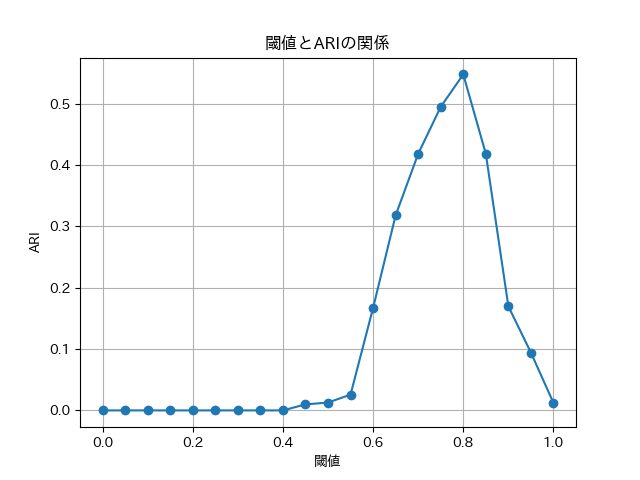
\includegraphics[scale=0.8]
    {contents/images/cw_graph.png}
  \caption{閾値ごとのARIの結果\label{fig:cw_graph}}
\end{figure}

このグラフより, 閾値を0.8としたときのARIが最も高くなることがわかった. したがって本研究では全てのデータのクラスタリングにおいて閾値は0.8に設定して行った. 

\subsection{他の手法との比較}
本研究で実装したChinese Whispersと, 一般的に使用されているクラスタリングであるK-Meansを比較する. まず, K-Meansはクラスタ数を事前に選択する必要があるためクラスタ数をいくつに設定すると最もARIが高くなるか検証した. 
クラスタ数とARIの関係を以下のグラフ\ref{fig:kmeans_graph}に示す.

\begin{figure}[hbtp]
  \centering
  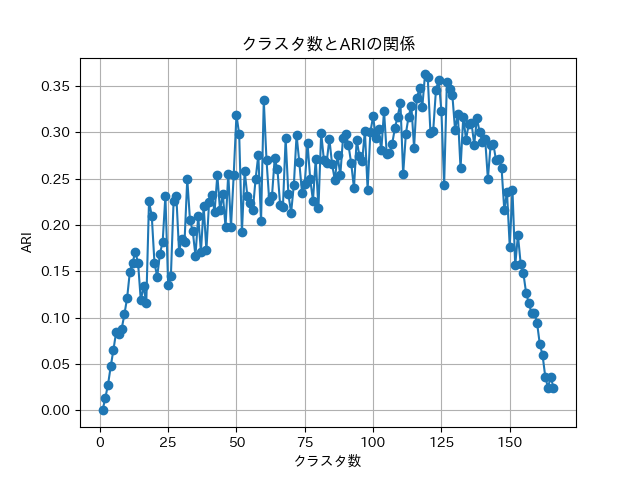
\includegraphics[scale=0.8]
    {contents/images/kmeans_graph.png}
  \caption{クラスタ数ごとのARIの結果\label{fig:kmeans_graph}}
\end{figure}

検証した結果, クラスタ数が126の時ARIは最も高い値を示した. 次にK-MeansとChinese Whispersの結果を比較した結果が以下の表\ref{tb:two_ari}である. 

\begin{table}[htbp]
  \caption{2つの手法におけるARI}
  \label{tb:two_ari}
  \begin{center}
  \begin{tabularx}{\linewidth}{|X|X|}
    \hline
    手法&ARIの最大値\\\hline\hline
    Chinese Whispers&0.5480604134843943\\\hline
    K-Means&0.3942834814562324\\\hline
  \end{tabularx}\end{center}
\end{table}

比較した結果, Chinese Whispersの方がARIが約0.15ほど高いことがわかった. 

\subsection{総評}
Chinese Whispersで作成されるグラフの閾値について検証した結果, 閾値を0.8としたときに最もARIが高い値を示すことがわかった. 
また, K-MeansとARIの最大値を比較した結果, Chinese Whispersの方がARIが高いことから本研究のクラスタリングの精度の高さを示すことができた. 
%ーーーーーーーーーーーーーーーーーーーーーーーーーーーー

% \section{RQ3:付与した各クラスタの名称は適切か}
% クラスタリング後の各クラスタの名称が適切なものとなっているか調査する. 

%ーーーーーーーーーーーーーーーーーーーーーーーーーーーー

\section{RQ3:可視化ツールの有用性はどうか}
\subsection{評価方法}
抽出, クラスタリングによって得られた結果を表示する可視化ツールについて調査する. 本研究で作成された可視化ツールの有用性に関して, 実験協力者にユーザビリティ, デザイン, 機能性の3点に関してアンケートをとり結果をまとめた. 

\subsection{結果}

\subsection{考察}

\subsection{総評}